\documentclass[11pt,a4paper]{report}
\usepackage[textwidth=37em,vmargin=30mm]{geometry}
\usepackage{calc,xunicode,amsmath,amssymb,paralist,enumitem,tabu,booktabs,datetime2,xeCJK,xeCJKfntef,listings}
\usepackage{tocloft,fancyhdr,tcolorbox,xcolor,graphicx,eso-pic,xltxtra,xelatexemoji}

\newcommand{\envyear}[0]{2025}
\newcommand{\envdatestr}[0]{2025-10-18}
\newcommand{\envfinaldir}[0]{webdb/2025/20251018/final}

\usepackage[hidelinks]{hyperref}
\hypersetup{
    colorlinks=false,
    pdfpagemode=FullScreen,
    pdftitle={Web Digest - \envdatestr}
}

\setlength{\cftbeforechapskip}{10pt}
\renewcommand{\cftchapfont}{\rmfamily\bfseries\large\raggedright}
\setlength{\cftbeforesecskip}{2pt}
\renewcommand{\cftsecfont}{\sffamily\small\raggedright}

\setdefaultleftmargin{2em}{2em}{1em}{1em}{1em}{1em}

\usepackage{xeCJK,xeCJKfntef}
\xeCJKsetup{PunctStyle=plain,RubberPunctSkip=false,CJKglue=\strut\hskip 0pt plus 0.1em minus 0.05em,CJKecglue=\strut\hskip 0.22em plus 0.2em}
\XeTeXlinebreaklocale "zh"
\XeTeXlinebreakskip = 0pt


\setmainfont{Brygada 1918}
\setromanfont{Brygada 1918}
\setsansfont{IBM Plex Sans}
\setmonofont{JetBrains Mono NL}
\setCJKmainfont{Noto Serif CJK SC}
\setCJKromanfont{Noto Serif CJK SC}
\setCJKsansfont{Noto Sans CJK SC}
\setCJKmonofont{Noto Sans CJK SC}

\setlength{\parindent}{0pt}
\setlength{\parskip}{8pt}
\linespread{1.15}

\lstset{
	basicstyle=\ttfamily\footnotesize,
	numbersep=5pt,
	backgroundcolor=\color{black!5},
	showspaces=false,
	showstringspaces=false,
	showtabs=false,
	tabsize=2,
	captionpos=b,
	breaklines=true,
	breakatwhitespace=true,
	breakautoindent=true,
	linewidth=\textwidth
}






\newcommand{\coverpic}[2]{
    % argv: itemurl, authorname
    Cover photo by #2~~(\href{#1}{#1})
}
\newcommand{\makeheader}[0]{
    \begin{titlepage}
        % \newgeometry{hmargin=15mm,tmargin=21mm,bmargin=12mm}
        \begin{center}
            
            \rmfamily\scshape
            \fontspec{BaskervilleF}
            \fontspec{Old Standard}
            \fontsize{59pt}{70pt}\selectfont
            WEB\hfill DIGEST
            
            \vfill
            % \vskip 30pt
            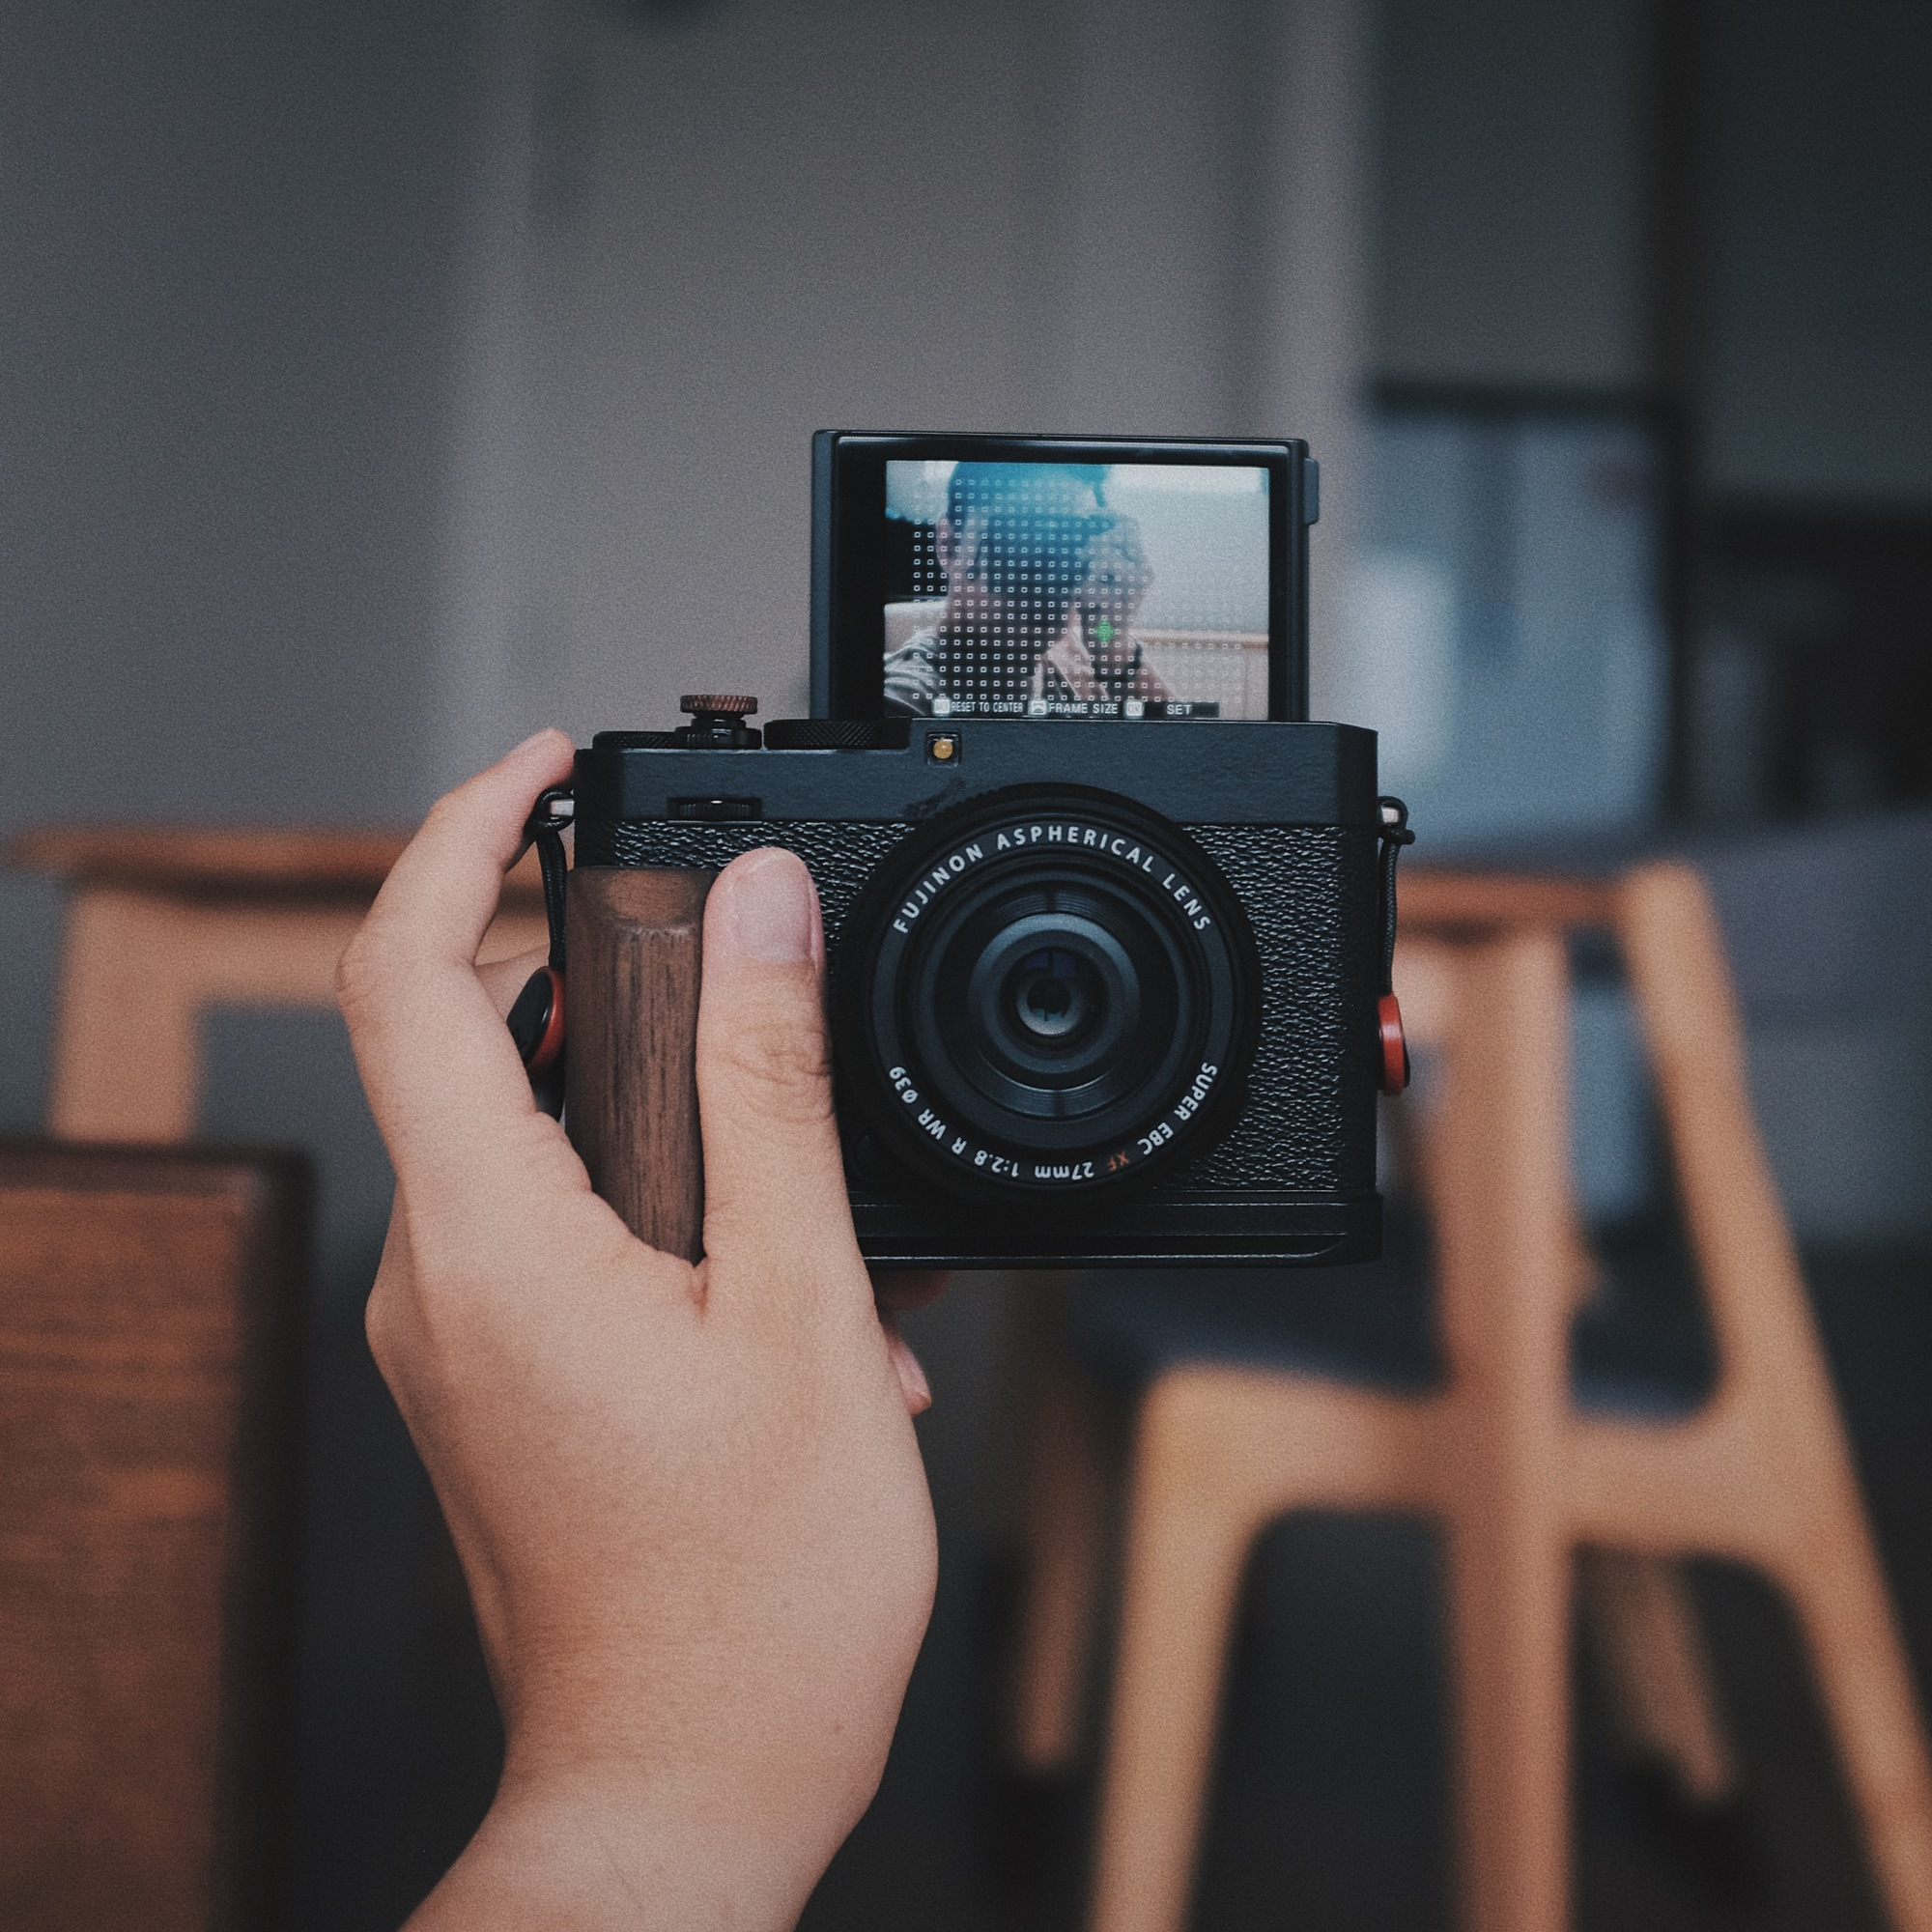
\includegraphics[width=\linewidth]{\envfinaldir/coverpic-prod.jpg}\par
            % \vskip 30pt
            \vfill

            \normalsize\rmfamily\scshape
            \copyright{} The Web Digest Project \hfill\large \envdatestr
        \end{center}
    \end{titlepage}
    % \restoregeometry
}
\newcommand{\simplehref}[1]{%
    \textcolor{blue!80!green}{\href{#1}{#1}}%
}
\renewcommand{\contentsname}{\center\Huge\sffamily\bfseries Contents\par\vskip 20pt}
\newcounter{ipartcounter}
\setcounter{ipartcounter}{0}
\newcommand{\ipart}[1]{
    % \vskip 20pt
    \clearpage
    \stepcounter{ipartcounter}
    \phantomsection
    \addcontentsline{toc}{chapter}{#1}
    % \begin{center}
    %     \Huge
    %     \sffamily\bfseries
    %     #1
    % \end{center}
    % \vskip 20pt plus 7pt
}
\newcounter{ichaptercounter}
\setcounter{ichaptercounter}{0}
\newcommand{\ichapter}[1]{
    % \vskip 20pt
    \clearpage
    \stepcounter{ichaptercounter}
    \phantomsection
    \addcontentsline{toc}{section}{\numberline{\arabic{ichaptercounter}}#1}
    \begin{center}
        \Huge
        \sffamily\bfseries
        #1
    \end{center}
    \vskip 20pt plus 7pt
}
\newcommand{\entrytitlefont}[1]{\subsection*{\raggedright\Large\sffamily\bfseries#1}}
\newcommand{\entryitemGeneric}[2]{
    % argv: title, url
    \parbox{\linewidth}{
        \entrytitlefont{#1}\par\vskip 5pt
        \footnotesize\ttfamily\mdseries
        \simplehref{#2}
    }\vskip 11pt plus 11pt minus 1pt
}
\newcommand{\entryitemGithub}[3]{
    % argv: title, url, desc
    \parbox{\linewidth}{
        \entrytitlefont{#1}\par\vskip 5pt
        \footnotesize\ttfamily\mdseries
        \simplehref{#2}\par\vskip 5pt
        \small\rmfamily\mdseries#3
    }\vskip 11pt plus 11pt minus 1pt
}
\newcommand{\entryitemAp}[3]{
    % argv: title, url, desc
    \parbox{\linewidth}{
        \entrytitlefont{#1}\par\vskip 5pt
        \footnotesize\ttfamily\mdseries
        \simplehref{#2}\par\vskip 5pt
        \small\rmfamily\mdseries#3
    }\vskip 11pt plus 11pt minus 1pt
}
\newcommand{\entryitemHackernews}[3]{
    % argv: title, hnurl, rawurl
    % \parbox{\linewidth}{
    %     \entrytitlefont{#1}\par\vskip 5pt
    %     \footnotesize\ttfamily\mdseries
    %     \simplehref{#3}\par
    %     \textcolor{black!50}{\href{#2}{#2}}
    % }\vskip 11pt plus 11pt minus 1pt
    \begin{minipage}{\linewidth}
            \entrytitlefont{#1}\par\vskip 5pt
            \footnotesize\ttfamily\mdseries
            \simplehref{#3}\par
            \textcolor{black!50}{\href{#2}{#2}}
    \end{minipage}\par\vskip 11pt plus 11pt minus 1pt
}







\begin{document}

\makeheader

\tableofcontents\clearpage




\ipart{Developers}
\ichapter{Hacker News}
\entryitemTwoLinks{US car repossessions surge as more Americans default on auto loans}{https://news.ycombinator.com/item?id=45622157}{https://www.theguardian.com/business/2025/oct/17/us-car-repossessions-economy}

\entryitemTwoLinks{The pivot}{https://news.ycombinator.com/item?id=45621074}{https://www.antipope.org/charlie/blog-static/2025/10/the-pivot-1.html}

\entryitemTwoLinks{GOG Has Had to Hire Private Investigators to Track Down IP Rights Holders}{https://news.ycombinator.com/item?id=45620394}{https://www.thegamer.com/gog-private-investigators-off-the-grid-ip-rights-holders/}

\entryitemTwoLinks{OpenAI Needs \$400B In The Next 12 Months}{https://news.ycombinator.com/item?id=45619544}{https://www.wheresyoured.at/openai400bn/}

\entryitemTwoLinks{Claude Skills are awesome, maybe a bigger deal than MCP}{https://news.ycombinator.com/item?id=45619537}{https://simonwillison.net/2025/Oct/16/claude-skills/}

\entryitemTwoLinks{Andrej Karpathy – AGI is still a decade away}{https://news.ycombinator.com/item?id=45619329}{https://www.dwarkesh.com/p/andrej-karpathy}

\entryitemTwoLinks{The Rapper 50 Cent, Adjusted for Inflation}{https://news.ycombinator.com/item?id=45618790}{https://50centadjustedforinflation.com/}

\entryitemTwoLinks{AI has a cargo cult problem}{https://news.ycombinator.com/item?id=45618350}{https://www.ft.com/content/f2025ac7-a71f-464f-a3a6-1e39c98612c7}

\entryitemTwoLinks{Dead or Alive creator Tomonobu Itagaki, 58 passes away}{https://news.ycombinator.com/item?id=45617986}{https://www.gamedeveloper.com/design/dead-or-alive-creator-tomonobu-itagaki-has-passed-away-at-58}

\entryitemTwoLinks{Intercellular communication in the brain through a dendritic nanotubular network}{https://news.ycombinator.com/item?id=45617819}{https://www.science.org/doi/10.1126/science.adr7403}

\entryitemTwoLinks{You did no fact checking, and I must scream}{https://news.ycombinator.com/item?id=45617088}{https://shkspr.mobi/blog/2025/10/i-have-no-facts-and-i-must-scream/}

\entryitemTwoLinks{Live Stream from the Namib Desert}{https://news.ycombinator.com/item?id=45615931}{https://bookofjoe2.blogspot.com/2025/10/live-stream-from-namib-desert.html}

\entryitemTwoLinks{Ruby core team takes ownership of RubyGems and Bundler}{https://news.ycombinator.com/item?id=45615863}{https://www.ruby-lang.org/en/news/2025/10/17/rubygems-repository-transition/}

\entryitemTwoLinks{A classified network of SpaceX satellites is emitting a mysterious signal}{https://news.ycombinator.com/item?id=45615481}{https://www.npr.org/2025/10/17/nx-s1-5575254/spacex-starshield-starlink-signal}

\entryitemTwoLinks{EVs are depreciating faster than gas-powered cars}{https://news.ycombinator.com/item?id=45615237}{https://restofworld.org/2025/ev-depreciation-blusmart-collapse/}

\entryitemTwoLinks{Migrating from AWS to Hetzner}{https://news.ycombinator.com/item?id=45614922}{https://digitalsociety.coop/posts/migrating-to-hetzner-cloud/}

\entryitemTwoLinks{Amazon's Ring to partner with Flock}{https://news.ycombinator.com/item?id=45614713}{https://techcrunch.com/2025/10/16/amazons-ring-to-partner-with-flock-a-network-of-ai-cameras-used-by-ice-feds-and-police/}

\entryitemTwoLinks{4Chan Lawyer publishes Ofcom correspondence}{https://news.ycombinator.com/item?id=45614148}{https://alecmuffett.com/article/117792}

\entryitemTwoLinks{Ask HN: How to stop an AWS bot sending 2B requests/month?}{https://news.ycombinator.com/item?id=45613567}{https://news.ycombinator.com/item?id=45613567}

\entryitemTwoLinks{Free the Internet: The Tor Project's annual fundraiser}{https://news.ycombinator.com/item?id=45613246}{https://blog.torproject.org/2025-fundraiser-donations-matched/}\ichapter{Phoronix}
\entryitemGeneric{\hskip 0pt{}GNOME Has A New Security Threat Scanner Powered By VirusTotal}{https://www.phoronix.com/news/GNOME-Lenspect-Threat-Scanner}

\entryitemGeneric{\hskip 0pt{}openSFI Is A Very Interesting Collaboration Between AMD \& Intel For Better Firmware Unification}{https://www.phoronix.com/news/openSFI}

\entryitemGeneric{\hskip 0pt{}Intel Introducing Microcode Staging Feature For Linux 6.19 To Cope With Bigger Blobs}{https://www.phoronix.com/news/Intel-Microcode-Staging-Linux}

\entryitemGeneric{\hskip 0pt{}Ubuntu 25.10 Performance On System76 Thelio Astra / Ampere Altra}{https://www.phoronix.com/review/ubuntu-2510-arm64}

\entryitemGeneric{\hskip 0pt{}AES-GCM Crypto Performance Up To ~74\% Faster For AMD Zen 3 With Linux 6.19}{https://www.phoronix.com/news/Linux-6.19-AES-GCM-AVX2-Faster}

\entryitemGeneric{\hskip 0pt{}New Linux Kernel Patches From Intel Delivering +18\% Database Performance}{https://www.phoronix.com/news/Linux-MM-CID-Faster-DBs}

\entryitemGeneric{\hskip 0pt{}Fedora Cloud Looks To Switch /boot To Btrfs Subvolume}{https://www.phoronix.com/news/Fedora-Cloud-Btrfs-Boot-Subvol}

\entryitemGeneric{\hskip 0pt{}Intel Vulkan Driver Adds Support For Xe Driver's Low Latency Hint}{https://www.phoronix.com/news/Intel-ANV-Xe-Low-Latency-Hint}

\entryitemGeneric{\hskip 0pt{}Linux Graphics Driver Fixes Readied For Linux 6.18-rc2}{https://www.phoronix.com/news/Linux-6.18-rc2-DRM-Fixes}


\ipart{Developers~~~~(zh-Hans)}
\ichapter{Solidot}
\entryitemGeneric{\hskip 0pt{}GZDoom 开源社区因创始人使用 AI 生成代码而分裂}{https://www.solidot.org/story?sid=82573}

\entryitemGeneric{\hskip 0pt{}韩国在四个月试用后放弃了 AI 教科书}{https://www.solidot.org/story?sid=82572}

\entryitemGeneric{\hskip 0pt{}南极洲冰盖出现类似格陵兰岛的加剧融化迹象}{https://www.solidot.org/story?sid=82571}

\entryitemGeneric{\hskip 0pt{}2024 年大气二氧化碳水平创新高}{https://www.solidot.org/story?sid=82570}

\entryitemGeneric{\hskip 0pt{}微软新产品计划在中国之外制造}{https://www.solidot.org/story?sid=82569}

\entryitemGeneric{\hskip 0pt{}Mozilla 测试免费的 Firefox VPN 服务}{https://www.solidot.org/story?sid=82568}

\entryitemGeneric{\hskip 0pt{}Paxos 不小心制造了 300 万亿美元的 PayPal 稳定币}{https://www.solidot.org/story?sid=82567}

\entryitemGeneric{\hskip 0pt{}Tor browser 移除 Firefox AI 功能}{https://www.solidot.org/story?sid=82566}

\entryitemGeneric{\hskip 0pt{}挪威实现电动汽车销售目标}{https://www.solidot.org/story?sid=82565}

\entryitemGeneric{\hskip 0pt{}日本政府要求 OpenAI 停止侵权}{https://www.solidot.org/story?sid=82564}

\entryitemGeneric{\hskip 0pt{}苹果新 MacBook Pro 电池续航力长达 24 小时}{https://www.solidot.org/story?sid=82563}

\entryitemGeneric{\hskip 0pt{}到 2050 年全球气温可能上升 2C}{https://www.solidot.org/story?sid=82562}

\entryitemGeneric{\hskip 0pt{}美国近七成成年人肥胖}{https://www.solidot.org/story?sid=82561}

\entryitemGeneric{\hskip 0pt{}Reddit 联合创始人称大部分互联网已死}{https://www.solidot.org/story?sid=82560}

\entryitemGeneric{\hskip 0pt{}GLP-1 减肥药有治疗糖尿病的潜力}{https://www.solidot.org/story?sid=82559}

\entryitemGeneric{\hskip 0pt{}美国近四成 2 岁以下儿童接触智能手机}{https://www.solidot.org/story?sid=82558}

\entryitemGeneric{\hskip 0pt{}苹果承诺增加在华投资}{https://www.solidot.org/story?sid=82557}

\entryitemGeneric{\hskip 0pt{}Firefox 145 Beta 停止发布 32 位 Linux 版本}{https://www.solidot.org/story?sid=82556}

\entryitemGeneric{\hskip 0pt{}黑客入侵安全公司窃取未披露漏洞信息和源代码}{https://www.solidot.org/story?sid=82555}

\entryitemGeneric{\hskip 0pt{}Firefox 144.0 释出}{https://www.solidot.org/story?sid=82554}\ichapter{V2EX}
\entryitemGeneric{\hskip 0pt{}[推广] 🔥「内购限免」👍一款美区超一万个好评的遥控,键盘\&鼠标应用。}{https://www.v2ex.com/t/1166553}

\entryitemGeneric{\hskip 0pt{}[问与答] 如何控制自我的情绪}{https://www.v2ex.com/t/1166551}

\entryitemGeneric{\hskip 0pt{}[Solana] 大家觉得 HyperLiquid 的代币\$HYPE 跌倒什么时候可以抄底? 20 美元以下?}{https://www.v2ex.com/t/1166550}

\entryitemGeneric{\hskip 0pt{}[生活] 分手了}{https://www.v2ex.com/t/1166549}

\entryitemGeneric{\hskip 0pt{}[加密货币] 强烈建议不要使用任何钱包生成的助记词,包括硬件钱包!}{https://www.v2ex.com/t/1166548}

\entryitemGeneric{\hskip 0pt{}[Linux] 有没有什么对 Linux 友好的主板}{https://www.v2ex.com/t/1166547}

\entryitemGeneric{\hskip 0pt{}[电影] 喜欢骑仿赛的程序员一定要去看《创:战神》,爽!}{https://www.v2ex.com/t/1166546}

\entryitemGeneric{\hskip 0pt{}[问与答] amazon.com 上如何买东西,邮寄到国内?}{https://www.v2ex.com/t/1166543}

\entryitemGeneric{\hskip 0pt{}[宽带症候群] [后续 3] 诉泉州联通案一审取得阶段性胜利,但仍需二审}{https://www.v2ex.com/t/1166542}

\entryitemGeneric{\hskip 0pt{}[Android] 港版哪些是双实体 sim 加 esim 机器}{https://www.v2ex.com/t/1166541}

\entryitemGeneric{\hskip 0pt{}[分享发现] B 站这抽奖是演都不演了}{https://www.v2ex.com/t/1166540}

\entryitemGeneric{\hskip 0pt{}[游戏] 五五开真的回来了吗?}{https://www.v2ex.com/t/1166539}

\entryitemGeneric{\hskip 0pt{}[分享发现] window11 居然自带剪贴板 历史了}{https://www.v2ex.com/t/1166537}

\entryitemGeneric{\hskip 0pt{}[宽带症候群] 深圳新装宽带 选哪家好}{https://www.v2ex.com/t/1166536}

\entryitemGeneric{\hskip 0pt{}[Linux] Linux 桌面没调好的,别怀疑,一定是技术没学到位}{https://www.v2ex.com/t/1166535}

\entryitemGeneric{\hskip 0pt{}[Android] 很好奇国内 Keep 运动的那个 App 他们是用 Android 原生开发的,还是用 Flutter 或者 RN 做的?}{https://www.v2ex.com/t/1166534}

\entryitemGeneric{\hskip 0pt{}[问与答] 求懂交通法的大佬分析一个交通事故案例}{https://www.v2ex.com/t/1166533}

\entryitemGeneric{\hskip 0pt{}[Apple] AppleTV 更新 26 后,遥控器``音量健''失灵了}{https://www.v2ex.com/t/1166532}

\entryitemGeneric{\hskip 0pt{}[小米] 说说雷布斯 ``云相册'' 真正智障的设定}{https://www.v2ex.com/t/1166531}

\entryitemGeneric{\hskip 0pt{}[问与答] 今年双十一哪里买 iPhone17 标准版便宜}{https://www.v2ex.com/t/1166528}

\entryitemGeneric{\hskip 0pt{}[Solana] 站长是否有必要干预 \$V2EX 的价格?}{https://www.v2ex.com/t/1166527}

\entryitemGeneric{\hskip 0pt{}[问与答] [请教]如何选购或组装台式电脑}{https://www.v2ex.com/t/1166524}

\entryitemGeneric{\hskip 0pt{}[问与答] 出北京地区京东洗衣和京东家政}{https://www.v2ex.com/t/1166522}

\entryitemGeneric{\hskip 0pt{}[iPhone] iOS 18 FaceTime 屏幕共享 变灰不可用是什么原因啊?}{https://www.v2ex.com/t/1166521}

\entryitemGeneric{\hskip 0pt{}[酷工作] [高薪 3.5w+]Web3 交易所招聘远程岗 Java 开发}{https://www.v2ex.com/t/1166520}

\entryitemGeneric{\hskip 0pt{}[OpenAI] 没忍住,对 GPT 爆粗口了,不知道 AI 统治人类的那天会不会被清算 :(}{https://www.v2ex.com/t/1166519}

\entryitemGeneric{\hskip 0pt{}[MIUI] 小米澎湃 2.0 如何禁用 guardprovider?}{https://www.v2ex.com/t/1166517}

\entryitemGeneric{\hskip 0pt{}[Solana] 81 号玩家大量减仓, 后续玩家排名+1}{https://www.v2ex.com/t/1166516}

\entryitemGeneric{\hskip 0pt{}[问与答] 关于北极航线}{https://www.v2ex.com/t/1166515}

\entryitemGeneric{\hskip 0pt{}[问与答] 咨询个问题我问 AI 写个 demo,怎么知道给我的 Demo 方向是正确的}{https://www.v2ex.com/t/1166514}

\entryitemGeneric{\hskip 0pt{}[问与答] Mac 上的看书/看漫画软件有推荐吗?(排除自带的图书 APP)}{https://www.v2ex.com/t/1166513}

\entryitemGeneric{\hskip 0pt{}[Apple] 被苹果的无线充电搞烦了,有没有有线充电底座类产品呀?}{https://www.v2ex.com/t/1166512}

\entryitemGeneric{\hskip 0pt{}[Linux] CentOS 之后,为什么你需要的是 AlmaLinux}{https://www.v2ex.com/t/1166511}

\entryitemGeneric{\hskip 0pt{}[Windows] office 365 版本的 onenote 终于有单元格合并功能了}{https://www.v2ex.com/t/1166510}

\entryitemGeneric{\hskip 0pt{}[问与答] 各位兄弟,你们软路由用的什么系统和什么梯子软件}{https://www.v2ex.com/t/1166509}

\entryitemGeneric{\hskip 0pt{}[酷工作] 游戏表现策划(远程)}{https://www.v2ex.com/t/1166508}

\entryitemGeneric{\hskip 0pt{}[问与答] 你们有什么好的方式扩展自己的见识、增长生活中的智慧吗??非常需要补充,如果有的话,请分享一下}{https://www.v2ex.com/t/1166507}

\entryitemGeneric{\hskip 0pt{}[程序员] 怎么评价 order by rand() limit 1 这条 sql}{https://www.v2ex.com/t/1166505}

\entryitemGeneric{\hskip 0pt{}[问与答] 在 MacOS 打开未知来源的 word 并且编辑,最坏的后果是什么?}{https://www.v2ex.com/t/1166503}

\entryitemGeneric{\hskip 0pt{}[问与答] 最近两周 OpenRouter 的免费模型在调用过程中,每次都会提示 429 错误,有遇到这个问题的吗}{https://www.v2ex.com/t/1166500}

\entryitemGeneric{\hskip 0pt{}[职场话题] 话说,有公司不提供纸巾的吗?}{https://www.v2ex.com/t/1166499}

\entryitemGeneric{\hskip 0pt{}[生活] 一件由于送礼引起的不愉快事件}{https://www.v2ex.com/t/1166497}

\entryitemGeneric{\hskip 0pt{}[macOS] 求助, macOS 究竟如何卸载微信输入法}{https://www.v2ex.com/t/1166495}

\entryitemGeneric{\hskip 0pt{}[问与答] 新凯来会发布光刻机吗?你们认为还要多久才能突破先进制程的光刻机?}{https://www.v2ex.com/t/1166493}

\entryitemGeneric{\hskip 0pt{}[问与答] 2025 年了 现在 windows 上可以正确播放杜比视界的方法还是没有吗? 除了自带电视和电影}{https://www.v2ex.com/t/1166491}

\entryitemGeneric{\hskip 0pt{}[骑行] 通勤业余自行车升级推荐}{https://www.v2ex.com/t/1166490}

\entryitemGeneric{\hskip 0pt{}[程序员] 大佬们,请教一个数据库设计的问题}{https://www.v2ex.com/t/1166489}

\entryitemGeneric{\hskip 0pt{}[OpenAI] 用美区 google play 礼品卡充值 chatgpt 的问题}{https://www.v2ex.com/t/1166488}

\entryitemGeneric{\hskip 0pt{}[汽车] 赛力斯董事长说:安全是最大的豪华,问界系列车型次年续保费用整体下降 30\%}{https://www.v2ex.com/t/1166487}

\entryitemGeneric{\hskip 0pt{}[分享发现] 现在普通的信息差还是很赚钱的。}{https://www.v2ex.com/t/1166485}


\ipart{Generic News}







\clearpage
\leavevmode\vfill
\footnotesize

Copyright \copyright{} 2023-2025 Neruthes and other contributors.

This document is published with CC BY-NC-ND 4.0 license.

The entries listed in this newsletter may be copyrighted by their respective creators.

This newsletter is generated by the Web Digest project.

The newsletters are also delivered via Telegram channel \CJKunderline{\href{https://t.me/webdigestchannel}{https://t.me/webdigestchannel}}.\\
RSS feed is available at \CJKunderline{\href{https://webdigest.pages.dev/rss.xml}{https://webdigest.pages.dev/rss.xml}}.

This newsletter is available in PDF at
\CJKunderline{\href{https://webdigest.pages.dev/}{https://webdigest.pages.dev/}}.

The source code being used to generate this newsletter is available at\\
\CJKunderline{\href{https://github.com/neruthes/webdigest}{https://github.com/neruthes/webdigest}}.

This newsletter is also available in
\CJKunderline{\href{http://webdigest.pages.dev/readhtml/\envyear/WebDigest-20251018.html}{HTML}} and
\CJKunderline{\href{https://github.com/neruthes/webdigest/blob/master/markdown/\envyear/WebDigest-20251018.md}{Markdown}}.


\coverpic{https://unsplash.com/photos/boombox-on-a-bicycle-mmRmFFZJcvI}{Ömer Haktan Bulut}


\end{document}
